\documentclass[11pt,spanish]{article}

\usepackage{listings}             
\usepackage{anysize} 
\usepackage{graphicx}
\usepackage[spanish]{babel}
\usepackage[utf8]{inputenc}
\usepackage{xcolor}
\usepackage{wrapfig}


\lstset{language=Python}
\marginsize{1cm}{1cm}{2cm}{2cm}
\selectlanguage{spanish}
\lstset{
language=Python,
 backgroundcolor=\color{red!75!green!50!blue!25},
 frame=single,
literate=
  {á}{{\'a}}1 {é}{{\'e}}1 {í}{{\'i}}1 {ó}{{\'o}}1 {ú}{{\'u}}1
  {Á}{{\'A}}1 {É}{{\'E}}1 {Í}{{\'I}}1 {Ó}{{\'O}}1 {Ú}{{\'U}}1
  {à}{{\`a}}1 {è}{{\`e}}1 {ì}{{\`i}}1 {ò}{{\`o}}1 {ù}{{\`u}}1
  {À}{{\`A}}1 {È}{{\'E}}1 {Ì}{{\`I}}1 {Ò}{{\`O}}1 {Ù}{{\`U}}1
  {ä}{{\"a}}1 {ë}{{\"e}}1 {ï}{{\"i}}1 {ö}{{\"o}}1 {ü}{{\"u}}1
  {Ä}{{\"A}}1 {Ë}{{\"E}}1 {Ï}{{\"I}}1 {Ö}{{\"O}}1 {Ü}{{\"U}}1
  {â}{{\^a}}1 {ê}{{\^e}}1 {î}{{\^i}}1 {ô}{{\^o}}1 {û}{{\^u}}1
  {Â}{{\^A}}1 {Ê}{{\^E}}1 {Î}{{\^I}}1 {Ô}{{\^O}}1 {Û}{{\^U}}1
  {œ}{{\oe}}1 {Œ}{{\OE}}1 {æ}{{\ae}}1 {Æ}{{\AE}}1 {ß}{{\ss}}1
  {ű}{{\H{u}}}1 {Ű}{{\H{U}}}1 {ő}{{\H{o}}}1 {Ő}{{\H{O}}}1
  {ç}{{\c c}}1 {Ç}{{\c C}}1 {ø}{{\o}}1 {å}{{\r a}}1 {Å}{{\r A}}1
  {€}{{\EUR}}1 {£}{{\pounds}}1
}


\title{\vspace{-3cm}\begin{flushleft}\textbf{Actividad 7}\end{flushleft}}
\author{\hspace{-9.6cm}\textsc{Andrés Ignacio Rodríguez Mendoza}}
\date{}

\begin{document}

\begin{wrapfigure}{r}{0.2\textwidth}
  \begin{center}
   \vspace{-5.4cm} 
\includegraphics[width=0.15\textwidth]{uni}
  \end{center}
\end{wrapfigure}

\maketitle  
\begin{center}
\rule{\textwidth}{1pt}
\end{center}

$$\alpha$$

\section*{Código}

\begin{lstlisting}

import numpy as np
from scipy import integrate
import pylab as p
import matplotlib.pyplot as plt


def pend(y, t):
    theta, omega = y
    return [omega, -(9.81)*np.sin(theta)]
    

# === Population equilibrium ===
# 
# Before using !SciPy to integrate this system, we will have a closer look on 
# position equilibrium. Equilibrium occurs when the growth rate is equal to 0.
# This gives two fixed points:

f2 = p.figure()


t= np.linspace(0, 7 * np.pi, 500)

X_f0 = np.array([-4*np.pi,2*np.pi])
X_f1 = np.array([1*np.pi,-0*np.pi])



values1 = np.linspace(-5.2, 2, 800)    
vcolors1= p.cm.Accent(np.linspace(-1, 1, len(values1)))

values2  = np.linspace(-8, 4, 200)    
vcolors2 = plt.cm.nipy_spectral(np.linspace(-0.51 , 0.93, len(values2)))


p.figure(2)


# plot trajectories
for v, col in zip(values1,vcolors1):
    X0 = v * X_f0                            # starting point
    X = integrate.odeint( pend, X0, t)       # we don't need infodict here
    plt.plot( X[:,0], X[:,1], lw=0.5*v, color=col)


#plot trajectories
for v, col in zip(values2, vcolors2):
    X1 = v * X_f1                            # starting point
    Y = integrate.odeint( pend, X1, t)       # we don't need infodict here
    plt.plot( Y[:,0], Y[:,1], lw=0.2*v, color=col)


plt.grid()
plt.xlim(-4*np.pi,4*np.pi)

plt.ylim(-10,10)


# define a grid and compute direction at each point



nb_points   = 20

x = np.linspace(-4*np.pi, 4*np.pi, nb_points)
y = np.linspace(-3*np.pi, 3*np.pi, nb_points)

X1 , Y1  = np.meshgrid(x, y)                       # create a grid


DX= pend([X1, Y1],t)                      # compute growth rate on the gridt

lw= 0.1*y/x


Q = plt.quiver(X1, Y1, DX[0], DX[1], DX, pivot='mid', cmap=plt.cm.cool, linewidth=lw)

p.title('Trayectorias y direcciones del campo')
p.xlabel('$\Theta$')
p.ylabel('$\omega$')
p.legend()
p.grid()


p.savefig('fase.png', dpi=200)




plt.show()
\end{lstlisting}

\section*{Gáficas}

\centering

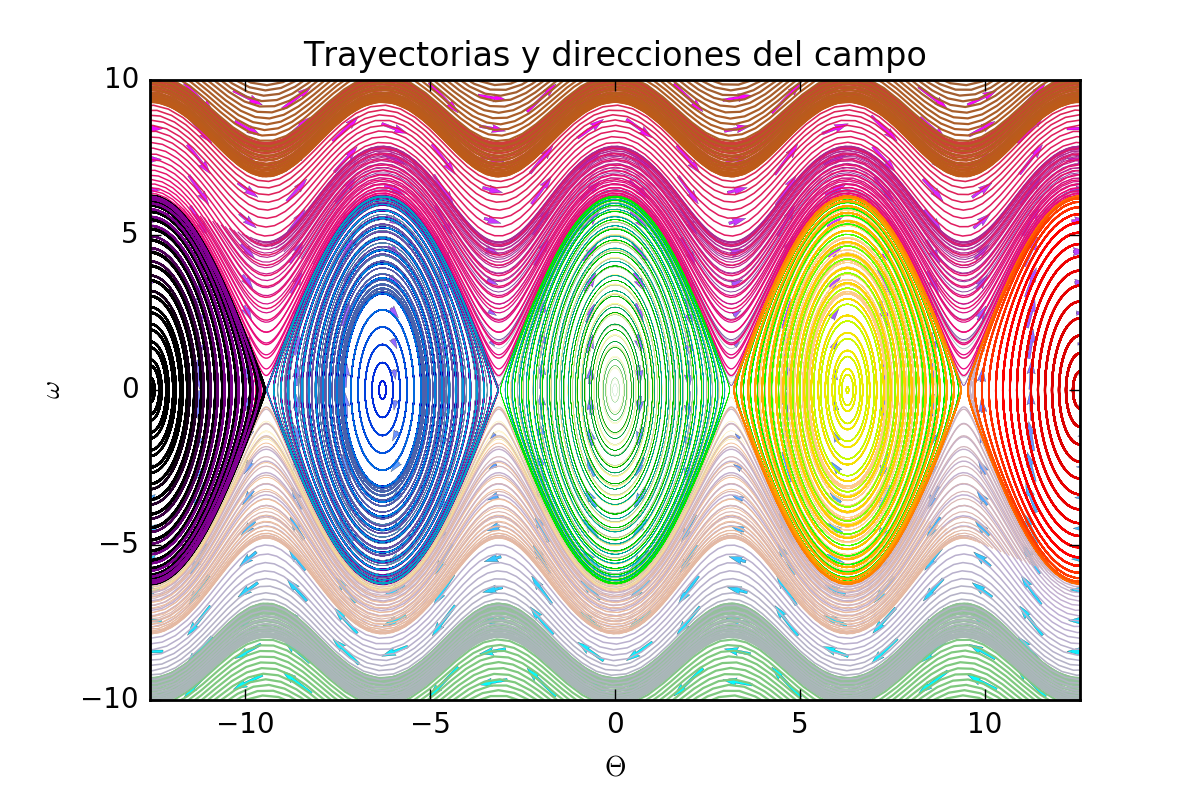
\includegraphics[scale=1.3]{fase}\\





\end{document}

